\chapterimage{Mavrica.jpg} % Chapter heading image

\chapter{Detektorji svetlobe}

Za konec bomo spoznali še detektorje svetlobe, ki so nepogrešljivi
pri kvantitativni obravnavi optičnih pojavov. Detektorji se med seboj razlikujejo
po svojih specifikacijah, ki jih bomo opisali v nadaljevanju, in po načinu delovanja. 
V grobem delimo detektorje na termične in kvantne. Podrobneje bomo spoznali nekaj vrst
termičnih in več vrst kvantnih detektorjev, predvsem polprevodniške fotodiode, in 
nazadnje spoznali šum, ki omejuje uporabnost naprav.

\section{Osnovne karakteristike detektorjev}

Osnovna naloga optičnih detektorjev je pretvoriti vpadni svetlobni signal 
v nek drug signal, ki ga lahko natančno merimo. Navadno sta to električni tok 
ali električna napetost, ki sta sorazmerna z intenziteto ali močjo vpadne svetlobe 
(in ne z amplitudo električne poljske jakosti). Omenili smo delitev detektorjev v dve skupini, 
ki loči detektorje na termične in kvantne. Prvi pretvorijo energijo vpadne svetlobe 
v toploto, drugi pa temeljijo na fotoefektu, kjer vpadli foton izbije elektron ali 
ustvari par elektron-vrzel.

Pri termičnih detektorjih zaznamo svetlobo tako,
da merimo povečanje temperature senzorja zaradi absorbirane svetlobe in taki detektorji
zaznavajo energijo vpadle svetlobe. Njihov odziv je razmeroma počasen, zato jih uporabljamo
predvsem za merjenje optične moči, po drugi strani pa neodvisen
od valovne dolžine vpadne svetlobe, zaradi česar so termični detektorji uporabni na 
širokem območju od globoke ultravijolične do daljne infrardeče svetlobe. Uporaba
prevlada predvsem v daljnem infrarfrečem območju, kjer drugi detektorji ne delujejo.
Primeri termičnih detektorjev so bolometer, termočlen in piroelektrični detektor.

Druga skupina so kvantni detektorji, v katerih se
fotoni absorbirajo in povzročijo pojav prostih nosilcev naboja. Taki detektorji
torej zaznavajo število vpadlih fotonov. Odlikuje jih zelo hiter odziv (pod $\si{\micro\second}$)
in pri velika občutljivost. Njihova slabost je omejen obseg valovnih dolžin,
pri katerih zaznavajo svetlobo, poleg tega jih je za optimalno delovanje treba 
hladiti. Primeri so vakuumske, polprevodniške in plazovne fotodiode.
\begin{figure}[h]
\centering
\def\svgwidth{65truemm} 
\input{slike/11_ShemaTermKv.pdf_tex}
\caption{Primerjava spektralnega odziva termičnega in kvantnega detektorja}
\label{fig:shemaTermKv}
\end{figure}

Osnovne karakteristike, ki omogočajo primerjavo med detektorji in določajo njihovo uporabnost,
so občutljivost, spektralni odziv, odzivni čas in prag detekcije. 

\begin{enumerate}
\item Občutljivost detektorja $R$ pove, koliko signala dobimo na enoto vpadnega svetlobnega toka. 
enota za občutljivost je tako A/W (ali tudi V/W). 
\item Spektralni odziv pove, kako se občutljivost spreminja z valovno dolžino $R(\lambda)$. 
Kvantni detektorji delujejo le v določenem območju valovnih dolžin, ki je odvisen od snovi, 
iz katere je detektor narejen. 
\item Odzivni čas pove, kako hitro se detektor odzove na spremembo optičnega signala. 
\item Prag detekcije pove, pri kolikšni vpadni svetlobni moči postane razmerje med signalom ($S$)
in šumom ($N$, {\it noise}) enako $S/N = 1$. 
\end{enumerate}

\section{Termični detektorji}
Uporaba termičnih detektorjev je precej omejena zaradi njihovega počasnega odziva. Zato
se večinoma uporabljajo za detekcijo svetlobe tistih valovnih dolžin, za katere ni drugih
preprostih ali učinkovitih detektorjev, ali pa v primeru, ko hitrega odziva ne potrebujemo.
Termični detektorji se zato danes uporabljajo predvsem v daljnem infrardečem, teraherčnem 
in mikrovalovnem območju, še posebej v astronomiji, in za termografske kamere.

Delovanje termičnih detektorjev temelji na spremembi temperature zaradi absorpcije svetlobe 
(energije), detektorji pa se med seboj razlikujejo predvsem v načinu pretvorbe spremembe 
temperature v električni signal.
Tipalo termičnih detektorjev mora biti pri vseh vrstah dobro počrnjeno, da absorbira
svetlobo v čim širšem spektralnem območju. Čeprav je njihova občutljivost načeloma 
neodvisna od valovne dolžine vpadne svetlobe, se v praksi pojavijo omejitve zaradi
prepustnosti okna in absorpcijskega spektra črnega nanosa. Tipala so majhna, zato 
da dosežemo čim hitrejši odziv, ki pa je kljub temu navadno počasnejši od 1~ms. 
Termične detektorje uporabljamo pri sobni temperaturi, za posebej zahtevne meritve pa 
jih lahko hladimo na nekaj K. 

Obravnavajmo termični detektor, katerega tipalo naj ima toplotno kapaciteto $C$. Toplota
se s tipala odvaja v nek toplotni rezervoar s temperaturo $T_0$, 
toplotne izgube pa označimo z $\Lambda$. Ko na tipalo vpada svetloba moč $P$, začne
temperatura tipala $T$ zaradi absorpcije svetlobe naraščati, hkrati pa se tipalo 
ohlaja zaradi odtekanja toplote:
\beq
\frac{dW}{dt} = C \frac{dT}{dt} = P - \Lambda (T-T_0).
\label{TD1}
\eeq
V stacionarnem stanju, ki ga dosežemo pri konstantnem vpadnem svetlobnem toku, se
temperatura tipala ne spreminja je enaka
\beq
T = T_0 + \frac{P}{\Lambda}.
\eeq
Občutljivost detektorja, ki je sorazmerna z razliko temperatur tipala in rezervoarja, 
je torej obratno sorazmerna z močjo, s katero se tipalo hladi. Toplotne izgube detektorja 
moramo torej kar se da zmanjšati. 

Iz enačbe~(\ref{TD1}) razberemo, 
da se temperatura približuje stacionarni vrednosti s časovno konstanto 
\beq
\tau = \frac{C}{\Lambda},
\label{TermD_t}
\eeq
ki je ključni parameter za določanje odzivnega časa detektorja. Vidimo, da je odzivni
čas sorazmeren s kapaciteto senzorja, zato so tipala praviloma zelo majhna.

Podrobneje poglejmo odziv termičnega detektorja od vpadne moči. Naj se vpadna moč
spreminja s časom, temperatura na detektorju pa temu sledi z določeno zakasnitvijo. Odziv
najlepše izračunamo v Fourierevem prostoru. Vpadna moč je tako
\beq
P(t) = \int_{-\infty}^{\infty} P_\omega e^{i\omega t}d\omega,
\eeq
temperatura pa
\beq
T = T_0 + \int_{-\infty}^{\infty} T_\omega e^{i\omega t}d\omega.
\label{TermTF}
\eeq
To vstavimo v enačbo~(\ref{TD1}) in dobimo
\beq
\int_{-\infty}^{\infty} i \omega T_\omega e^{i\omega t}d\omega = \frac{1}{C}
\int_{-\infty}^{\infty} (P_\omega - \Lambda T_\omega) e^{i\omega t}d\omega.
\eeq
Enačbi zadostimo, če izenačimo člene pred vsako spektralno komponento posebej
\beq
i \omega T_\omega = \frac{1}{C}\left(P_\omega - \Lambda T_\omega\right).
\eeq
Sledi 
\beq
T_\omega = \frac{1}{\Lambda}\left(\frac{1}{1+i \omega \tau}\right)P_\omega,
\label{TermOdziv}
\eeq
pri čemer je $\tau$ odzivni čas (enačba~\ref{TermD_t}). Sprememba temperature
je tako obratno sorazmerna s toplotnimi izgubami, zato moramo za čim večji 
odziv detektorja izgube čim bolj zmanjšati. Pri tem hlajenje s prevajanjem toplote
razmeroma preposto zmanjšamo, ne moremo pa zmanjšati toplotnih izgub s sevanjem.
Najmanjše toplotne izgube so tako podane kar s Stefanovim zakonom. Če majhne izgube
povečajo občutljivost, pa p drugi strani podaljšajo karakteristični čas $\tau$, 
zato pri termičnih detektorjih ne moremo imeti hkrati močnega in hitrega odziva. 

\begin{definition}
Pokaži, da je odziv termičnega detektorja na zelo kratek svetlobni sunek oblike 
$P(t) = P_0 \delta(t-t_0)$ enak 
\beq
T(t)=\frac{iP_0}{\Lambda}e^{-(t-t_0)/\tau}.
\eeq
\end{definition}

\subsection*{Bolometer}
Bolometer je termični detektor, pri katerem zaznavamo spremembo električne upornosti
zaradi spremembe temperature tipala. Tipalo je praviloma počrnjena tanka ploščica, 
navadno je narejena iz termistorja, polprevodnika ali superprevodnika. Tipalo preko
referenčnega upora priključimo na napetost, preko kondenzatorja pa merimo napetost na njem.
Za meritve konstantega svetlobnega toka tipalo navadno vežemo v Wheatstonov mostiček. V obeh
primerih za referenčni upor vzamemo kar enako tipalo, ki ga zaščitimo pred vpadno svetlobo, 
tako da postane sistem neobčutljiv na morebitne spremembe temperature okolice.
\begin{figure}[h]
\centering
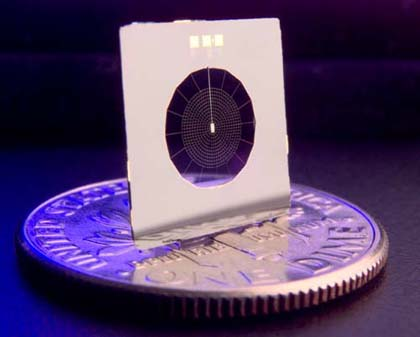
\includegraphics[width=90truemm]{slike/11_Bolometer.jpg}
\caption{Bolometer za merjenje prasevanja. Premer kovanca za primerjavo je 18~mm. 
Vir: NASA/JPL-Caltech.}
\label{fig:Bolometer}
\end{figure}

Pri bolometrih s termistorjem velja približno linearna zveza med upornostjo in 
temperaturo, vendar spremembe niso zelo velike, zato taki detektorji niso zelo 
občutljivi (nekaj $\%/\si{\kelvin}$ oziroma $R\sim 100~\si{\volt/\watt}$). 
So pa robustni, stabilni in delujejo pri sobni 
temperaturi. Odzivni časi so okoli $\tau \sim 1-20~\si{\milli\second}$. Pri polprevodniških
bolometrih upornost narašča eksponentno s temperaturo. Pogosto uporabljamo germanijev
bolometer, ki pa mora biti hlajen s tekočim helijem. Tako lahko dosežemo
občutljivosti $R \sim 10^8~\si{\volt/\watt}$. Zelo občutljivi so tudi 
detektorji s superprevodnimi tipali, saj je odvisnost upornosti od temperature v bližini
prehoda v superprevodno stanje zelo velika ($R \sim 10^3~\si{\volt/\watt}$).

\subsection*{Termočlen}
Termočlen je sestavljen iz dveh različnih vodnikov. En spoj vodnikov počrnimo, drugega, 
referenčnega, pa zaščitimo pred svetlobo. Zaradi vpadne svetlobe se počrnjeni spoj 
segreje, med obema spojema nastane temperaturna razlika in zaradi termoelektričnega 
pojava tudi električna napetost, ki jo lahko merimo. Pri tem pazimo, da je prevodnost
vodnikov čim večja, toplotna prevodnost pa čim manjša. Odzivni čas termočlenov je 
okoli $\tau \sim 10-20~\si{\milli\second}$, občutljivost pa je $R \sim 10~\si{\volt/\watt}$.
Ker so napetosti, ki se pojavijo med stikoma, razmeroma majhne (le okoli 
$\sim 10~\si{\micro\volt/K}$) pogosto vežemo več termočlenov zaporedno v termobaterijo, navadno
nekaj deset. Občutljivost s tem naraste na $R \sim 200~\si{\volt/\watt}$, podaljša 
pa se časovna konstanta $\tau \sim 10-2000~\si{\milli\second}$.

\subsection*{Piroelektrični detektor}
Piroelektriki so snovi brez centra inverzije, v katerih je lastna električna 
polarizacija odvisna od temperature (npr. LiTaO$_3$, triglicin sulfat TGS ali
polivinilidenfluorid, PVDF). 
Vsi feroelektriki so tudi piroelektriki. Piroelektrični detektor je narejen iz 
ploščice piroelektrične snovi med dvema elektrodama oziroma ploščama kondenzatorja.
Ko se ploščica zaradi absorbirane svetlobe segreje, se ji spremeni polarizacija in 
med elektrodama se pojavi premikalni tok, ki ga merimo na merilnem uporniku.

Zveza med spremembo temperature in spremembo polarizacije je
\beq
dP = a dT,
\eeq
kjer je $a$ piroelektrični koeficient. Med obema elektrodama s površino $S$ preteče naboj
\beq
de = I dt = S dP = S a dT.
\eeq
Tok skozi tipalo je tako
\beq
I = S a \frac{dT}{dt}.
\label{piro}
\eeq
Piroelektrični detektor je torej občutljiv na časovni odvod temperature detektorja, 
s tem pa tudi na spreminjanje vpadne svetlobne moči. V stacionarnem stanju 
detektor ne proizvaja električnega toka, zato moramo za merjenje 
konstantnega svetlobnega toka vpadno svetlobo najprej periodično modulirati.
Navadno to naredimo kar z mehanskim zaklopom. Piroelektrični detektorji
se uporabljajo kot dokaj ceneni in enostavni infrardeči detektorji, tudi v IR kamerah. 
Njihova občutljivost je $R \sim 1~\si{\micro\ampere/\watt}$, odzivni čas pa odvisen od 
upornika v vezju, ampak lahko doseže vrednosti $\tau \sim 10~\si{\micro\second}$.
Zavedati se je treba, da so piroelektrični koeficienti navadno močno 
odvisni od temperature in naraščajo do faznega prehoda pri Curiejevi temperaturi, 
pri kateri spontana polarizacija snovi izgine. 

Poglejmo temperaturni odziv na tipalu. Izhajamo iz enačb~(\ref{TermTF}), (\ref{TermOdziv}) in
(\ref{piro}) in izračunajmo tok $I$ vo odvisnosti od frekvence modulacije.
\beq
I = Sa \frac{dT}{dt} = Sa \frac{d}{dt} \int_{-\infty}^{\infty} T_\omega e^{i\omega t}d\omega 
=Sa\int_{-\infty}^{\infty}\frac{1}{\Lambda}\left(\frac{P_\omega}{1+i \omega \tau}\right) \,i \omega\,
e^{i\omega t}d\omega.
\eeq
Sledi 
\beq
I_\omega = \frac{i \omega\, SaP_\omega/\Lambda}{1 + i \omega \tau}.
\eeq
Vidimo, da pri majhnih frekvencah tok narašča, pri velikih frekvencah pa postane neodvisen od
frekvence modulacije vpadne svetlobe. Vendar to še ne pomeni, da lahko moduliramo s poljubno 
veliko frekvenco. Poleg relaksacijskega časa detektorja ima namreč karakteristični čas tudi
elektronsko vezje, ki določa zgornjo mejo za frekvenco. Ta je enak $\tau_e = R_eC_e$, pri čemer
sta $R_e$ upornost sistema in $C_e$ kapaciteta detektorja. 
\begin{figure}[h]
\centering
\def\svgwidth{90truemm} 
\input{slike/11_Piro.pdf_tex}
\caption{Spektralni odziv piroelektričnega detektorja. Karakteristični čas odziva je 
določen s toplotnimi izgubami $\Lambda$ in toplotno kapaciteto detektorja $C$, navzgor
pa odziv omejuje odziv elektronskega vezja $\tau_e$.}
\label{fig:Piro}
\end{figure}

\begin{definition}
Piroelektrični detektor naredimo iz kristala LiTaO$_3$ s koeficientom piroelektričnosti
$a = 2,3 \times 10^{-4}~\si{\ampere \second /\metre^2 \kelvin}$ in povprečno 
dielektričnostjo $\varepsilon = 50$. Izračunaj dovoljeno električno upornost sistema, 
če želimo, da detektor dobro deluje za frekvence do 1~MHz. 
Dimenzija detektorja je $S = 1~\si{\centi\metre^2}$ in debelina $d = 1~\si{\milli\metre}$.
\end{definition}

\section{Fotoefekt}
Delovanje kvantnih detektorjev temelji na fotoefektu, pri katerem vpadli
foton iz kovine izbije elektrone (fotoelektrone). Pri fotoefektu s svetlobo
dane valovne dožine osvetlimo katodo, nato pa merimo tok, ki teče med katodo
in anodo pri dani napetosti. S spreminjanjem napetosti lahko izmerimo kinetično 
energijo fotoelektronov, ki so izstopili iz kovine. Izkaže se, da pri določenih 
valovnih dolžinah svetlobe tok fotoelektronov povsem izgine, ne glede na moč vpadne svetlobe.
Fotoelektroni nastanejo le, če je energija vpadnih fotonov večja od izstopnega
dela kovine. Fotoefekt je prvič opazil Hertz leta 1887, razložil pa ga
je Einstein leta 1905 in zanj dobil nobelovo nagrado. 
\begin{figure}[h]
\centering
\def\svgwidth{65truemm} 
\input{slike/11_Fotoefekt.pdf_tex}
\caption{Shema fotocelice, v kateri poteka fotoefekt. 
Vpadna svetloba iz katode izbije elektrone, da med katodo in anodo steče tok.}
\label{fig:Fotoefekt}
\end{figure}

Poglejmo uporabnost fotoefekta za optično detekcijo. Glavna omejitev je 
izstopno delo snovi, na katero vpada svetloba. Za kovine je izstopno delo $\Phi$
od okoli 2~eV za cezij pa do okoli 6~eV za platino. 
Ustrezna valovna dolžina svetlobe, ki še povzroči fotoefekt, je tako 
\beq
\lambda \leq \frac{hc}{\Phi},
\eeq
kar je 640~nm za primer cezija in samo okoli 200~nm za platino. Če želimo ta pojav
izkostisti za detektorje, območje občutljivosti povečamo z uporabo drugih snovi,
na primer kompozitnih materialov (Cs-Te, Cs-Sb, Na-K-Sb-Cs) ali polprevodnikov (GaAs:Cs).
Izstopno delo s tem zmanjšamo na $\Phi \sim 0,7$~eV, tako da lahko zaznavamo 
vpadne fotone z valovnimi dolžinami od ultravijolične svetlobe pa vse do infrardeče. 

Omenimo še enkrat, da je pri detektorjih, ki temeljijo na fotoefektu
(kvantnih detektorjih), odziv sorazmeren s številom vpadnih fotonov in ne energijo 
vpadne svetlobe. V idealnem primeru je tako spektralni odziv konstanen, 
če gledamo na število vpadlih fotonov, in linearno
narašča z valovno dolžino, če gledamo na moč vpadne svetlobe.

Beseda fotoefekt je prvotno označevala opisan pojav: izbijanje elektronov iz snovi. 
Pojem pa lahko razširimo na pojav, pri katerem izbiti elektron ne zapusti snovi, 
ampak zgolj preide iz enega energijskega pasu v drugega. Pri tem zaradi
absorpcije fotona nastane par elektron-vrzel, prag za nastanek para pa je določen
z režo med energijskima nivojema. Prvemu pojavu zato pravimo zunanji fotoefekt, 
drugemu pa notranji fotoefekt. Primeri detektorjev, ki temeljijo na zunanjem fotoefektu, so 
fotocelice in fotopomnoževalke, detektorjev, ki temeljijo na notranjem fotoefektu, pa
fotoprevodniki, polprevodniške in plazovne fotodiode.


\section{Vakuumska fotodioda in fotopomnoževalka}

Najpreprostejši kvantni detektor na zunanji fotoefekt je fotocelica (slika~\ref{fig:Fotoefekt}). 
Svetloba vpada na fotokatodo, ki je zaprta v vakuumirani stekleni bučki, in tam povzroči
fotoefekt. Fotoelektrone, ki zapustijo katodo, z zunanjo napetostjo potegnemo na anodo 
in merimo električni tok. 

Da je čas preleta
elektronov od katode do anode čim krajši, je napetost na fotocelici pogosto nekaj kilovoltov.
Tedaj je lahko odzivni čas okoli 0,1~ns. Enostavnost in hitrost so torej prednosti fotocelice, slaba
stran pa majhna občutljivost.

PMT 0,9A/W, 0.2-1.1 mum, dc-1Ghz
celica 0.001 A/W isto.

termally generated atoms -> noise; cooling. 

Pomemeben podatek za kvantne detektorje, ki je v tesni zvezi 
z občutljivostjo, je tudi kvantni izkotiste, to je delež vpadlih fotonov, ki povzročijo fotoefekt.


\section{Fotopomnoževalka}
Fotopomnoževalke so fotocelice z vgrajenim ojačevanjem. Fotoelektron pospešimo z napetostjo
okoli 100-150~V na vmesno elektrodo - dinodo, kjer izbije nekaj (3-5) sekundarnih elektronov. 
Pomnoževanje se ponovi 8-14 krat, tako da dobimo na en fotoelektron na anodi $10^6 - 10^8$ 
elektronov, česar ni težko zaznati. Fotopomnoževalkanasm tako omogoča štetje posameznih fotonov.
Za manj zahtevne aplikacije pa pogosto merimo kar povprečni tok z anode. Zaravi delikega ojačenje
je treba tudi paziti, da fotopomnoževalke ne osvetlimo preveč. Spektralna občutljivost
tako fotocelice kot fotopomnoževalke je odvisna od sestave površine fotokatode. Večinoma
je največja v modrem delu spektra. Spodnja meja delovanja fotopomnoževalk je okoli $1~\si{\micro\metre}$.
Kvantni izkoristek je večinoma okoli $10~\%$, razen v bližnjem infrardečem območju, kjer
je znantno manjši. 

Ojačanje ne poslabša S/N ratio. 


\section{Fotoprevodni detektorji}
V fotoprevodnikih svetloba z dovolj veliko energijo tvori pare elektron-vrzel, zaradi  česar
se poveča število nosilcev toka in s tem prevodnost. Hitrost odziva je odvisna od hitrosti
rekombinacije elektronov in vrzeli, to je okoli mikrosekunde po do desetin milisekund, kar
je dokaj počasi. 

\section{PN in PiN fotodiode}
Polvodniški detektroji so dveh vrst: fotoprevodniki in diodni. Spektralna občutljivost
obojih je odvisna od velikosti energijske reže emd valenčnim in prevodnim pasom. Silicij
z energijsko režo 1~eV je uporaben do valovne dolžine 1,2 mikron, germanij pa do 1,6 mikron.
V vidnem in bližnjem infrardečem področju deluje še GaAs, CdS in PbS, zadnja dva le kot
fotoprevodnika. Kot fotoprevodniki pri večjih valovnih dolžinah se uporabljajo  še PbTe
in HgCdTe. Posebej zadni je zelo pomemben, ker ima pri pravem razmerju Hg in Cd vrh občutljivosti
pri okoli 10 mikronov, to je ravno pri vrhu sevanja črnega telesa s temperaturo okoli 300~K. 
Z ustreznim doziranjem pa lahko polvodniški fotoprevodniki delujejo do valovnih dolžin nekaj 100 mikronov.
Detektorje  z majhno energijso režo je treba hladiti, navadno s tekočim dušikom, da zmanjšamo
termično vzbujanje elektronov v prevodni pas. Pri energiji fotonov blizu energijske reže 
imajo polvodniški detektorji zelo velik kvantni izkoriste, kar blizu 1.

Fotodiode zaznajo le pare elektron-vrzel v območju izpraznjenega sloja p-n spoja. Električno 
polje v tem sloju povzroči, da elektron odteče na eno stran, vrzel pa na drugo. Fotodopda tako
generira tok, ki je sorazmeren z vpadlo svetlobno močjo. Zaradi nelinearne zveze med tokom in napetostjo
na diodi je treba skrbeti, da je napetost na diodi vselej 0 ali celo v zaporni smeri, kar lahko
dosežemo z zunanjo napetostjo v zaporni smeri. S tem tudi dosežemo hitrejši odziv, ker 
se zmajša kapacitivnost p-n spoja. 

Da se bo svetloba absorbirala ravno v p-n spoju, mora biti seveda spoj pri površini dopde, obenem
pa mora biti spoj čim debelejši, kar dosežejo s tem, da je med  p in n stranjo še plast
čistega polvodnika. Takim diodam pravimo pin diode. 

V pn spoju je mooče doseči tudi pomnoževanje nastalih elektronov in vrzeli, če je zaporna napetost dovolj 
velika, da lahko fotoelektron dobi toliko energije, preden zapusti izpraznjeni sloj, da tvori nove pare.
Taka pomnoževalna dioda je zelo občutljiva, vendar ima tudi večji šum.

\section{Plazovne fotodiode}
 
\section{CCD in CMOS detektorji}
 
\section{Šum pri optični detekciji}
Sama občutljivost nekega detektorja, to je količina A/W za neko fotodiodo, nam ne pove, kolikšen 
je najmanjši signal, ki ga je mogoče meriti. Ta je določen s šumom detektorja in pa s časom 
meritve, to je s frekvenčno širino modulacije svetlobe, ki jo želimo meriti. Največja 
možna frekvencčna širina je seveda določena s hitrostjo odziva detektorja.

Ocenimo fluktuacije, torej šum, toka nekega detektorja, na primer fotodiode. V času
meritve $\tau$ steče $n$ elektronov. Tok je torej
\beq
I = ne/\tau.
\eeq
Povprečni tok je seveda
\beq
\overline{I} = \overline{n}e/\tau.
\eeq
Napravimo mnogo meritev, vse dolge $\tau$. Ker so posamezni foto dogodki med seboj neodvisni, 
lahko predpostavimo, da je porazdelitev pretečenih elektronov Poissonova: pa lahko izračunamo
povprečni kvadrat fluktuacij toka
\beq
\sigma^2 = \overline{(I-\overline{I})^2} = \frac{e^2}{\tau^2} \overline{(n-\overline{n})^2} = 
\frac{e^2}{\tau^2}\overline{n} = \frac{e\overline{I}}{\tau}.
\eeq
Tokovni šum je obratno sorazmeren korenu iz časa merjenja, oziroma sorazmeren s korenom
iz širine merjenjega frekvenčnega intervala. Najmanjši povprečni tok diode je tok zaradi
termičnega vzbujanja, s tem je seveda po enačbi določen tudi osnovni termični šum diode.
Temni tok diode je sorazmeren s površino diode in eksponentno odvisen od temperature in 
energijske reže polvodnika;
\beq
I_0 = Sj_0 e^{-E_g/kT}
\eeq
Tipičen temni tok silicijeve fotodiode s površino 1~mm$^2$ je pri sobni temperaturi 1~nA. 
Tokovni šum je torej po gornji enačbi
\beq
I_N = \sqrt{eI_0\Delta \nu} \approx 10^{-15}~A/\sqrt{Hz} \sqrt{\Delta \nu}.
\eeq

Svetlobni tok, označen pogosto z NEP (noise equivalent power), ki da enak signal, je $10^4 $
fotonov na sekundo ali $10^{-14}$~W. Še beseda o enoti za NEP. Navadno je podan na enoto 
frekvenčnega intervala, to je po enačbi .. na $\sqrt{Hz}$. 